\documentclass[11pt,a4paper]{article}
\usepackage[utf8]{inputenc}
\usepackage[T1]{fontenc}
\usepackage[french]{babel}
\usepackage{geometry}
\usepackage{graphicx}
\usepackage{hyperref}
\usepackage{enumitem}
\usepackage{listings}
\usepackage{xcolor}
\usepackage{amsmath}
\usepackage{url}
\geometry{margin=2.5cm}

% Configuration pour les blocs de code
\lstset{
    basicstyle=\ttfamily\small,
    breaklines=true,
    frame=single,
    backgroundcolor=\color{gray!10},
    language=JavaScript,
    keywordstyle=\color{blue},
    commentstyle=\color{green!60!black},
    stringstyle=\color{red},
    numbers=left,
    numberstyle=\tiny\color{gray}
}

\title{Projet R\&D -- Pullman Concept Room\\\large Système d'authentification automatisée pour chambre intelligente\\\normalsize Rapport technique détaillé}
\author{Ethan Binisti -- ESILV A5}
\date{Février 2026}

\begin{document}

\maketitle

\tableofcontents
\newpage

\section{Introduction}

\subsection{Contexte du projet}

Accor, leader mondial de l'hôtellerie, souhaite moderniser l'expérience client dans ses hôtels Pullman en développant un système d'authentification sans contact pour les chambres. L'objectif est de permettre aux clients d'ouvrir leur chambre directement depuis leur smartphone, sans avoir besoin de clé physique ou de carte magnétique.

Ce projet de recherche et développement vise à créer une \textbf{maquette fonctionnelle} complète d'un système de gestion de chambres intelligentes, depuis le check-in jusqu'à l'ouverture de porte, en passant par la gestion des accès et la sécurité.

\subsection{Objectifs principaux}

Les objectifs de ce projet sont multiples :

\begin{itemize}
    \item \textbf{Sécuriser l'authentification} : Créer un système de tokens (clés numériques) sécurisés et temporaires pour chaque client
    \item \textbf{Anonymiser les données} : Protéger les informations personnelles des clients tout en permettant l'authentification
    \item \textbf{Simplifier l'expérience client} : Réduire les actions physiques nécessaires (plus besoin de passer à la réception, plus de clé à perdre)
    \item \textbf{Gérer les accès} : Permettre la gestion centralisée de toutes les chambres depuis un tableau de bord (GRMS)
    \item \textbf{Traçabilité} : Enregistrer tous les événements (check-in, tentatives d'ouverture, intrusions) dans des logs
    \item \textbf{Préparer l'intégration BLE} : Créer une architecture prête pour une future intégration Bluetooth Low Energy (BLE) avec iOS
\end{itemize}

\section{Architecture générale du système}

\subsection{Vue d'ensemble}

Le système est composé de \textbf{quatre composants principaux} qui communiquent entre eux :

\begin{enumerate}
    \item \textbf{GRMS API} : Le serveur backend qui gère toute la logique métier
    \item \textbf{Dashboard Web} : L'interface d'administration pour le personnel de l'hôtel
    \item \textbf{Room Core} : Le système embarqué dans chaque chambre (simulé par un serveur Node.js)
    \item \textbf{Application iOS Client} : L'application mobile pour les clients
\end{enumerate}

\subsection{Schéma de communication}

Le flux de communication suit ce schéma (représenté avec des flèches simples pour rester lisible dans le PDF) :

\begin{center}
\begin{tabular}{c}
\textbf{Client iOS (Smartphone)} \\
\\
$\downarrow$ \small JWT Auth \& Token Request \\
\\
\textbf{GRMS API (Backend)} \hspace{1cm} $\leftrightarrow$ \hspace{1cm} \textbf{Dashboard Web (Admin)} \\
\\
$\downarrow$ \small Token Verification \\
\\
\textbf{Room Core (Raspberry Pi)} \\
\end{tabular}
\end{center}

\subsection{Technologies utilisées}

\subsubsection{Backend (GRMS API)}

\begin{itemize}
    \item \textbf{Node.js} : Environnement d'exécution JavaScript côté serveur
    \item \textbf{Express} : Framework web minimaliste pour créer des APIs REST
    \item \textbf{JSON Web Token (JWT)} : Système d'authentification sécurisé
    \item \textbf{CORS} : Mécanisme pour autoriser les requêtes cross-origin
\end{itemize}

\textbf{Pourquoi ces technologies ?}
\begin{itemize}
    \item Node.js permet d'utiliser JavaScript aussi bien côté client que serveur, facilitant le développement
    \item Express est simple, léger et parfait pour créer rapidement une API REST
    \item JWT permet une authentification stateless (sans session serveur), idéale pour les applications mobiles
\end{itemize}

\subsubsection{Frontend Web (Dashboard)}

\begin{itemize}
    \item \textbf{React} : Bibliothèque JavaScript pour créer des interfaces utilisateur
    \item \textbf{Vite} : Outil de build ultra-rapide pour le développement
    \item \textbf{JavaScript (ES6+)} : Langage de programmation moderne
\end{itemize}

\textbf{Pourquoi React ?}
\begin{itemize}
    \item React permet de créer des interfaces réactives qui se mettent à jour automatiquement
    \item Composants réutilisables facilitent la maintenance du code
    \item Grande communauté et nombreux outils disponibles
\end{itemize}

\subsubsection{Room Core (Simulation)}

\begin{itemize}
    \item \textbf{Node.js} : Même environnement que le backend pour la cohérence
    \item \textbf{Express} : Pour créer un mini-serveur HTTP dans chaque chambre
    \item \textbf{Axios} : Bibliothèque pour faire des requêtes HTTP vers le GRMS
\end{itemize}

\subsubsection{Application iOS}

\begin{itemize}
    \item \textbf{Swift} : Langage de programmation officiel d'Apple pour iOS
    \item \textbf{SwiftUI} : Framework moderne d'Apple pour créer des interfaces
    \item \textbf{CoreBluetooth} : Framework pour la communication BLE (prévu pour la suite)
    \item \textbf{URLSession} : API native pour les requêtes HTTP
\end{itemize}

\textbf{Pourquoi Swift et SwiftUI ?}
\begin{itemize}
    \item Swift est le langage natif recommandé par Apple pour iOS
    \item SwiftUI permet de créer des interfaces modernes avec moins de code
    \item Performance optimale sur les appareils Apple
\end{itemize}

\section{Description détaillée des composants}

\subsection{GRMS API (Backend)}

\subsubsection{Rôle et responsabilités}

Le GRMS API est le \textbf{cœur du système}. Il centralise toute la logique métier :

\begin{itemize}
    \item Gestion des clients et de leurs données
    \item Gestion des réservations
    \item Génération et validation des tokens d'accès
    \item Gestion de l'état des chambres (libre, occupée, verrouillée)
    \item Enregistrement de tous les événements dans des logs
    \item Authentification JWT pour sécuriser l'accès à l'application mobile
\end{itemize}

\subsubsection{Structure des données}

Le système utilise un \textbf{stockage en mémoire} (pour la maquette). En production, ces données seraient stockées dans une base de données.

\paragraph{Clients}
Chaque client est représenté par :
\begin{itemize}
    \item \texttt{id} : Identifiant unique
    \item \texttt{name} : Nom du client
    \item \texttt{email} : Adresse email (utilisée pour l'authentification)
    \item \texttt{password} : Mot de passe hashé (pour l'authentification JWT)
    \item \texttt{phone} : Numéro de téléphone (optionnel)
    \item \texttt{status} : Statut du client
\end{itemize}

\paragraph{Chambres}
Chaque chambre contient :
\begin{itemize}
    \item \texttt{id} : Numéro de la chambre (ex: 101, 102)
    \item \texttt{status} : État actuel (\texttt{free}, \texttt{occupied}, \texttt{locked})
    \item \texttt{lockedUntil} : Date jusqu'à laquelle la chambre est verrouillée (en cas d'intrusion)
\end{itemize}

\paragraph{Tokens}
Les tokens sont des clés numériques temporaires :
\begin{itemize}
    \item \texttt{value} : Valeur aléatoire unique du token (ex: "101-1771317699037-ycx1pqo0c9")
    \item \texttt{clientId} : ID du client propriétaire
    \item \texttt{roomId} : Numéro de la chambre concernée
    \item \texttt{valid} : Booléen indiquant si le token est toujours valide
    \item \texttt{validFrom} : Date de début de validité (timestamp)
    \item \texttt{validTo} : Date de fin de validité (timestamp)
\end{itemize}

\paragraph{Réservations}
Les réservations lient clients et chambres :
\begin{itemize}
    \item \texttt{id} : Identifiant unique
    \item \texttt{clientId} : ID du client
    \item \texttt{roomId} : Numéro de la chambre
    \item \texttt{startDate} : Date de début du séjour
    \item \texttt{endDate} : Date de fin du séjour
    \item \texttt{status} : État (\texttt{pending}, \texttt{in\_progress}, \texttt{completed})
\end{itemize}

\paragraph{Logs}
Chaque événement est enregistré :
\begin{itemize}
    \item \texttt{id} : Identifiant unique
    \item \texttt{type} : Type d'événement (\texttt{CHECKIN}, \texttt{AUTH\_ATTEMPT}, \texttt{CHECKOUT}, etc.)
    \item \texttt{roomId} : Chambre concernée
    \item \texttt{timestamp} : Date et heure de l'événement
    \item \texttt{payload} : Données supplémentaires (JSON)
\end{itemize}

\subsubsection{Endpoints principaux}

\paragraph{Authentification}
\begin{itemize}
    \item \texttt{POST /auth/login} : Connexion d'un client avec email/mot de passe, retourne un JWT
    \item \texttt{GET /auth/me} : Vérifie le JWT et retourne les informations du client connecté
    \item \texttt{GET /auth/my-token} : Récupère le token actif pour le client connecté
\end{itemize}

\paragraph{Gestion des chambres}
\begin{itemize}
    \item \texttt{GET /rooms} : Liste toutes les chambres et leur état
    \item \texttt{POST /rooms/:id/unlock} : Déverrouille une chambre verrouillée
\end{itemize}

\paragraph{Check-in et Check-out}
\begin{itemize}
    \item \texttt{POST /checkin} : Génère un token, occupe la chambre, crée un log
    \item \texttt{POST /checkout} : Libère la chambre, invalide les tokens
\end{itemize}

\paragraph{Gestion des tokens}
\begin{itemize}
    \item \texttt{POST /tokens/verify} : Vérifie si un token est valide pour une chambre donnée
\end{itemize}

\paragraph{Clients}
\begin{itemize}
    \item \texttt{GET /clients} : Liste tous les clients
    \item \texttt{POST /clients} : Crée un nouveau client
\end{itemize}

\paragraph{Réservations}
\begin{itemize}
    \item \texttt{GET /reservations} : Liste toutes les réservations
    \item \texttt{POST /reservations} : Crée une nouvelle réservation
    \item \texttt{POST /reservations/:id/checkin} : Effectue un check-in depuis une réservation
\end{itemize}

\paragraph{Logs}
\begin{itemize}
    \item \texttt{GET /logs} : Récupère les logs récents
    \item \texttt{POST /room-events} : Enregistre un événement depuis le room-core
\end{itemize}

\subsubsection{Sécurité}

\paragraph{Authentification JWT}
Le système utilise JSON Web Tokens pour authentifier les clients sur l'application mobile. Le processus est le suivant :

\begin{enumerate}
    \item Le client se connecte avec son email et mot de passe via \texttt{POST /auth/login}
    \item Le serveur vérifie les identifiants
    \item Si valides, le serveur génère un JWT contenant l'ID du client et une date d'expiration
    \item Le JWT est renvoyé au client et stocké dans l'application mobile
    \item Pour chaque requête suivante, le client envoie le JWT dans l'en-tête \texttt{Authorization: Bearer <token>}
    \item Le serveur vérifie la signature et la validité du JWT avant de traiter la requête
\end{enumerate}

\paragraph{Validation des tokens}
Avant d'autoriser l'ouverture d'une porte, le système vérifie :
\begin{itemize}
    \item Que le token existe dans la base de données
    \item Que le token est associé à la bonne chambre
    \item Que le token est toujours valide (\texttt{valid = true})
    \item Que la date actuelle est entre \texttt{validFrom} et \texttt{validTo}
    \item Que la chambre n'est pas verrouillée pour intrusion
\end{itemize}

\paragraph{Détection d'intrusion}
Si plusieurs tentatives d'authentification échouent consécutivement (3 échecs), le système :
\begin{itemize}
    \item Verrouille la chambre (\texttt{status = "locked"})
    \item Enregistre un événement \texttt{INTRUSION\_LOCK} dans les logs
    \item Empêche toute nouvelle tentative pendant 2 minutes
    \item Notifie le personnel via le dashboard
\end{itemize}

\subsection{Dashboard Web (Interface d'administration)}

\subsubsection{Rôle}

Le dashboard web est l'\textbf{interface d'administration} utilisée par le personnel de l'hôtel pour :
\begin{itemize}
    \item Visualiser l'état de toutes les chambres en temps réel
    \item Effectuer les check-in et check-out
    \item Gérer les clients et leurs réservations
    \item Consulter les logs d'activité
    \item Gérer les situations d'urgence (déverrouillage de chambres)
\end{itemize}

\subsubsection{Structure de l'interface}

L'interface est organisée en plusieurs sections :

\paragraph{Section Check-in}
Permet de :
\begin{itemize}
    \item Sélectionner un client dans une liste déroulante
    \item Choisir une chambre disponible
    \item Définir la durée de validité du token (en minutes)
    \item Générer le token et effectuer le check-in
    \item Libérer la chambre (check-out)
\end{itemize}

\paragraph{Section Chambres}
Affiche :
\begin{itemize}
    \item Toutes les chambres avec leur statut visuel (couleur)
    \item Le nombre de chambres libres, occupées, verrouillées
    \item Un bouton pour simuler une tentative d'accès (pour les tests)
\end{itemize}

\paragraph{Section Clients \& Réservations}
Permet de :
\begin{itemize}
    \item Créer de nouveaux clients (fichier client)
    \item Voir la liste des clients existants
    \item Créer des réservations (client + chambre + dates)
    \item Effectuer un check-in anticipé depuis une réservation
\end{itemize}

\paragraph{Section Logs}
Affiche en temps réel :
\begin{itemize}
    \item Tous les événements récents (check-in, tentatives d'accès, intrusions, etc.)
    \item Le type d'événement, la chambre concernée, le succès/échec, l'heure
    \item Filtrage possible par type d'événement
\end{itemize}

\subsubsection{Captures d'écran du dashboard GRMS}

Pour illustrer concrètement l'outil d'administration, les figures suivantes montrent le dashboard en situation réelle :

\begin{figure}[h]
    \centering
    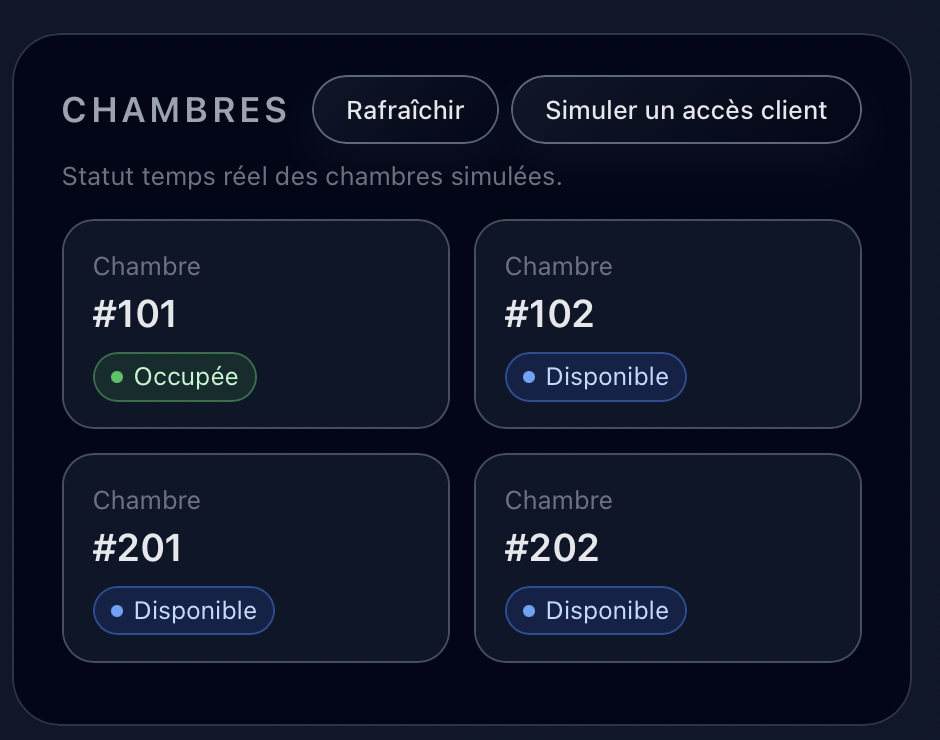
\includegraphics[width=0.9\textwidth]{images/grms-clients-reservations.png}
    \caption{Vue ``Chambres'' du dashboard GRMS : affichage en temps réel du statut des chambres (disponible, occupée, etc.).}
    \label{fig:grms-rooms}
\end{figure}

\begin{figure}[h]
    \centering
    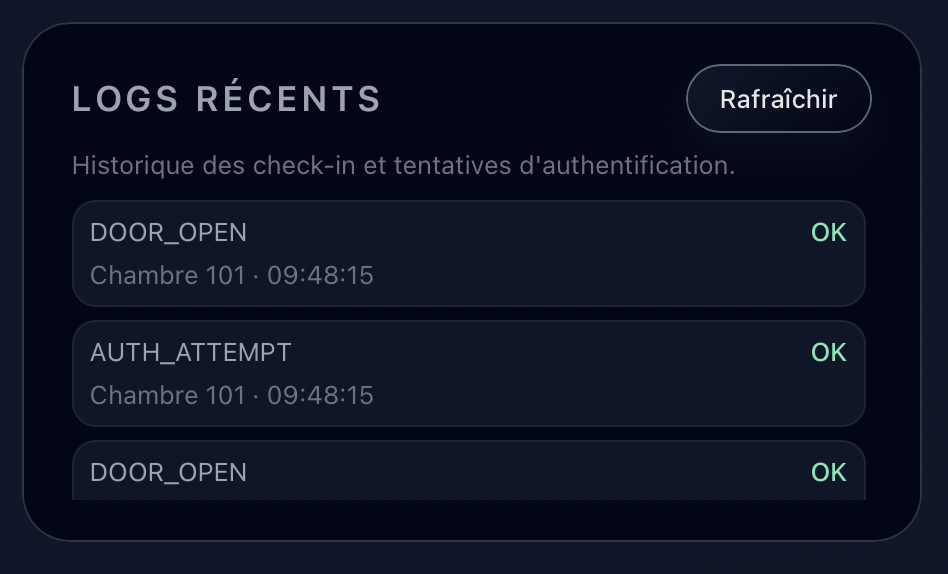
\includegraphics[width=0.9\textwidth]{images/ios-login.png}
    \caption{Vue ``Logs récents'' du dashboard GRMS : historique des ouvertures de porte et tentatives d'authentification.}
    \label{fig:grms-logs}
\end{figure}

\subsubsection{Fonctionnement technique}

Le dashboard est une \textbf{application React} qui :
\begin{itemize}
    \item Se connecte au GRMS API via des requêtes HTTP
    \item Met à jour automatiquement l'interface quand les données changent
    \item Utilise des appels \texttt{fetch()} pour communiquer avec le backend
    \item Affiche les données en temps réel grâce au rafraîchissement automatique
\end{itemize}

\subsection{Room Core (Cœur de chambre)}

\subsubsection{Rôle}

Le Room Core simule le système embarqué qui serait installé dans chaque chambre (typiquement un Raspberry Pi). Il représente le \textbf{point d'entrée physique} de la chambre.

\subsubsection{Fonctionnalités}

\paragraph{Authentification locale}
\begin{itemize}
    \item Reçoit les tentatives d'authentification depuis le smartphone du client
    \item Vérifie le token avec le GRMS API
    \item Gère un compteur local d'échecs consécutifs
    \item Peut se verrouiller localement en cas de trop d'échecs
\end{itemize}

\paragraph{Simulation d'ouverture de porte}
\begin{itemize}
    \item Simule l'ouverture de la porte électronique
    \item Enregistre l'événement dans le GRMS
    \item Gère l'état de la porte (ouverte, fermée, verrouillée)
\end{itemize}

\paragraph{Sécurité locale}
\begin{itemize}
    \item Maintient un verrouillage local temporaire après 3 échecs
    \item Communique avec le GRMS pour signaler les intrusions
    \item Peut être déverrouillé à distance depuis le dashboard
\end{itemize}

\subsubsection{Communication avec le GRMS}

Le Room Core communique avec le GRMS via HTTP :
\begin{itemize}
    \item \texttt{POST /tokens/verify} : Vérifie un token avec le GRMS
    \item \texttt{POST /room-events} : Envoie des événements (ouverture de porte, verrouillage) au GRMS
\end{itemize}

\subsection{Application iOS Client}

\subsubsection{Rôle}

L'application iOS est l'\textbf{interface client} qui permet aux clients de :
\begin{itemize}
    \item Se connecter avec leurs identifiants
    \item Récupérer automatiquement leur clé numérique après le check-in
    \item Ouvrir leur chambre en approchant leur smartphone du lecteur
\end{itemize}

\subsubsection{Architecture de l'application}

L'application est structurée selon le pattern \textbf{MVVM} (Model-View-ViewModel) :

\paragraph{Modèles (Models)}
\begin{itemize}
    \item \texttt{User} : Structure représentant un utilisateur (id, name, email)
    \item \texttt{TokenResponse} : Structure pour la réponse contenant le token
\end{itemize}

\paragraph{Vues (Views)}
\begin{itemize}
    \item \texttt{ContentView} : Interface principale avec deux vues :
    \begin{itemize}
        \item Vue de connexion (login)
        \item Vue principale (affichage de la clé, bouton d'ouverture)
    \end{itemize}
\end{itemize}

\paragraph{ViewModels}
\begin{itemize}
    \item \texttt{ClientViewModel} : Gère l'état de l'application et la logique métier
\end{itemize}

\paragraph{Services}
\begin{itemize}
    \item \texttt{AuthService} : Gère l'authentification JWT et le stockage local
    \item \texttt{ApiClient} : Gère toutes les communications HTTP avec le GRMS et le Room Core
\end{itemize}

\subsubsection{Captures d'écran de l'application iOS}

Les figures suivantes présentent l'écran principal de l'application client iOS ainsi qu'un rappel visuel du parcours clé numérique :

\begin{figure}[h]
    \centering
    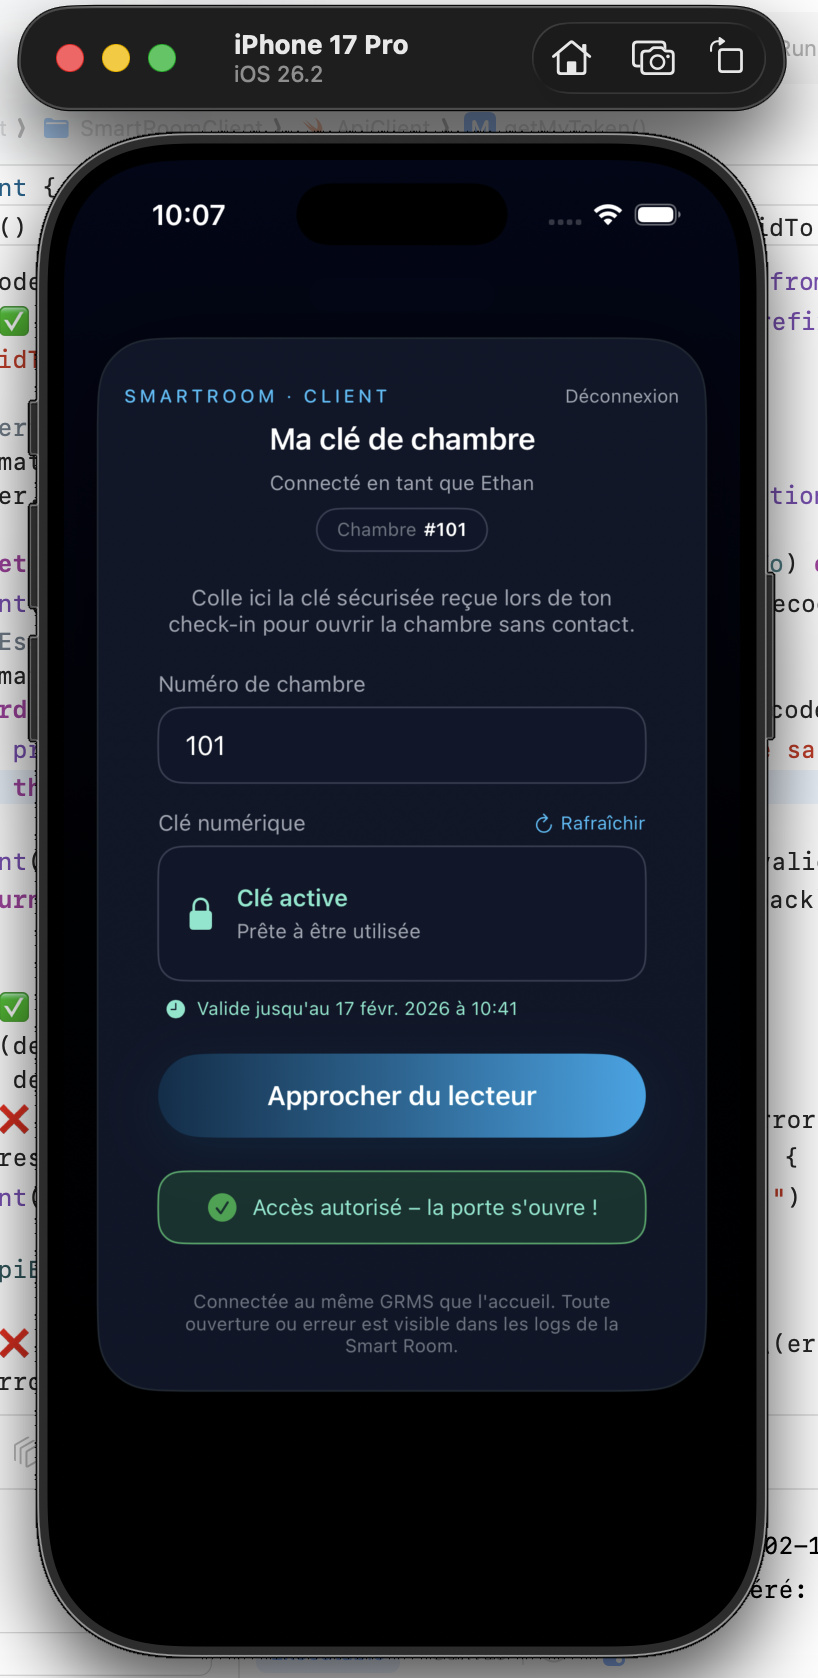
\includegraphics[width=0.6\textwidth]{images/grms-dashboard-rooms.png}
    \caption{Écran principal de l'application iOS : clé numérique active pour la chambre, date de validité et bouton ``Approcher du lecteur''.}
    \label{fig:ios-main}
\end{figure}

\begin{figure}[h]
    \centering
    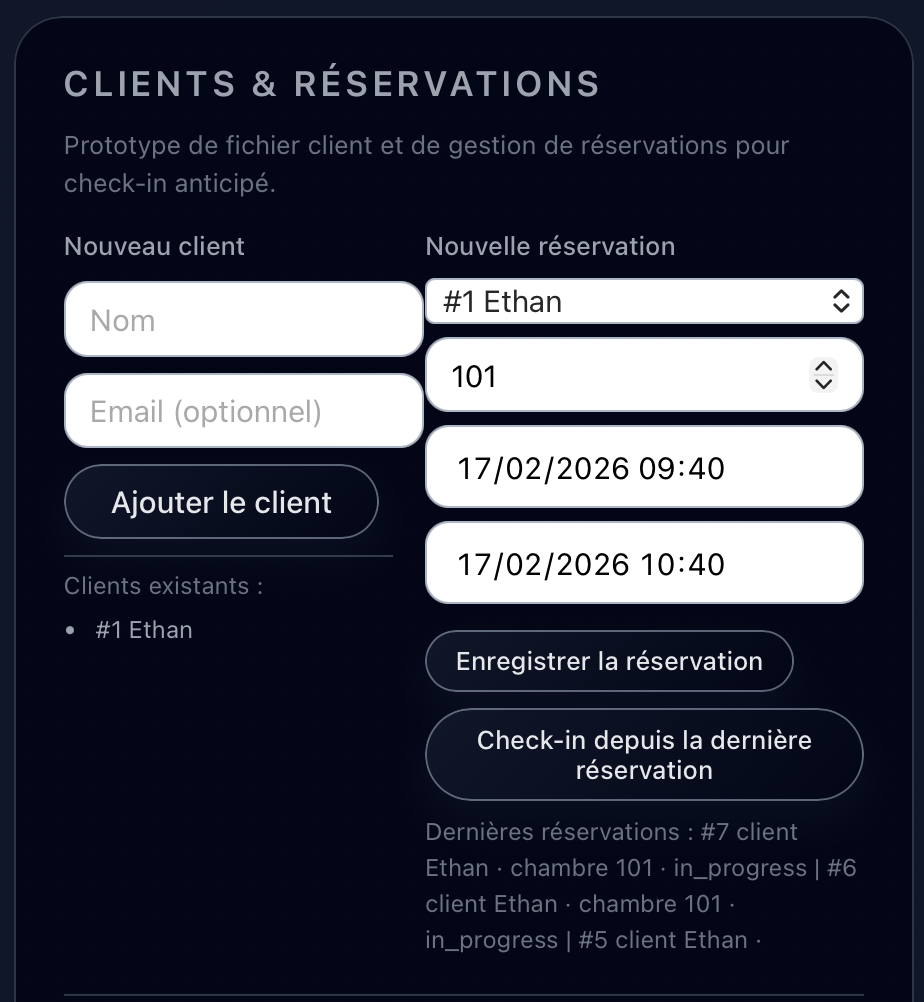
\includegraphics[width=0.6\textwidth]{images/ios-main-key.png}
    \caption{Rappel visuel du lien entre l'application iOS et le GRMS : la clé numérique est issue d'un check-in côté accueil (clients \& réservations).}
    \label{fig:ios-key-flow}
\end{figure}

\subsubsection{Fonctionnement détaillé}

\paragraph{Connexion}
\begin{enumerate}
    \item L'utilisateur entre son email et mot de passe
    \item L'application envoie une requête \texttt{POST /auth/login} au GRMS
    \item Le GRMS vérifie les identifiants et retourne un JWT
    \item L'application stocke le JWT dans \texttt{UserDefaults} (stockage local iOS)
    \item L'application récupère automatiquement le token actif via \texttt{GET /auth/my-token}
\end{enumerate}

\paragraph{Récupération du token}
\begin{enumerate}
    \item Après connexion, l'application appelle automatiquement \texttt{GET /auth/my-token}
    \item Le GRMS vérifie le JWT et retourne le token actif pour ce client
    \item Le token est stocké dans le ViewModel (mais \textbf{non affiché} à l'utilisateur pour la sécurité)
    \item La date de validité est affichée à l'utilisateur
\end{enumerate}

\paragraph{Ouverture de porte}
\begin{enumerate}
    \item L'utilisateur appuie sur "Approcher du lecteur"
    \item L'application envoie le token au Room Core via \texttt{POST /auth}
    \item Le Room Core vérifie le token avec le GRMS
    \item Si valide, le Room Core simule l'ouverture de la porte
    \item L'application affiche un message de succès
\end{enumerate}

\subsubsection{Sécurité dans l'application}

\paragraph{Stockage sécurisé}
\begin{itemize}
    \item Le JWT est stocké dans \texttt{UserDefaults}, qui est chiffré par iOS
    \item Le token de chambre n'est \textbf{pas affiché} à l'utilisateur (masqué pour la sécurité)
    \item Seul un indicateur visuel (cadenas) indique si une clé est active
\end{itemize}

\paragraph{Authentification}
\begin{itemize}
    \item Toutes les requêtes vers le GRMS incluent le JWT dans l'en-tête \texttt{Authorization}
    \item Le JWT expire après un certain temps (configuré dans le GRMS)
    \item En cas d'expiration, l'utilisateur doit se reconnecter
\end{itemize}

\section{Parcours utilisateur complet}

\subsection{Scénario type : Check-in et ouverture de porte}

Voici le parcours complet d'un client depuis son arrivée jusqu'à l'ouverture de sa chambre :

\subsubsection{Étape 1 : Réservation (avant l'arrivée)}

\begin{enumerate}
    \item Le personnel de l'hôtel crée une réservation dans le dashboard
    \item La réservation lie un client à une chambre pour des dates données
    \item Le statut de la réservation est \texttt{pending} (en attente)
\end{enumerate}

\subsubsection{Étape 2 : Check-in anticipé}

\begin{enumerate}
    \item Le personnel peut effectuer un check-in anticipé depuis le dashboard
    \item Le système génère un token valide pour la période du séjour
    \item La chambre passe en statut \texttt{occupied}
    \item Un événement \texttt{CHECKIN\_FROM\_RESERVATION} est enregistré dans les logs
\end{enumerate}

\subsubsection{Étape 3 : Arrivée du client}

\begin{enumerate}
    \item Le client ouvre l'application iOS sur son smartphone
    \item Il se connecte avec son email et mot de passe (créés lors de la réservation)
    \item L'application authentifie le client et récupère un JWT
    \item L'application récupère automatiquement le token actif pour sa chambre
    \item L'application affiche un indicateur visuel (cadenas vert) indiquant qu'une clé est active
    \item La date de validité est affichée
\end{enumerate}

\subsubsection{Étape 4 : Ouverture de la porte}

\begin{enumerate}
    \item Le client se rend devant sa chambre
    \item Il ouvre l'application et appuie sur "Approcher du lecteur"
    \item L'application envoie le token au Room Core de la chambre
    \item Le Room Core vérifie le token avec le GRMS
    \item Si valide, le Room Core simule l'ouverture de la porte
    \item Un événement \texttt{DOOR\_OPEN} est enregistré dans les logs
    \item L'application affiche "Accès autorisé – la porte s'ouvre !"
\end{enumerate}

\subsubsection{Étape 5 : Check-out}

\begin{enumerate}
    \item À la fin du séjour, le personnel effectue le check-out depuis le dashboard
    \item Le système invalide tous les tokens de la chambre
    \item La chambre repasse en statut \texttt{free}
    \item Un événement \texttt{CHECKOUT} est enregistré
    \item Le client ne peut plus ouvrir la chambre (son token est invalidé)
\end{enumerate}

\subsection{Scénario d'intrusion}

Si quelqu'un tente d'ouvrir une chambre sans autorisation :

\begin{enumerate}
    \item Une tentative d'authentification avec un token invalide est effectuée
    \item Le Room Core vérifie avec le GRMS et reçoit une réponse négative
    \item Le compteur local d'échecs est incrémenté
    \item Après 3 échecs consécutifs, le Room Core se verrouille localement
    \item La chambre passe en statut \texttt{locked} dans le GRMS
    \item Un événement \texttt{INTRUSION\_LOCK} est enregistré
    \item Le personnel est alerté via le dashboard
    \item La chambre reste verrouillée pendant 2 minutes minimum
    \item Le personnel peut déverrouiller manuellement depuis le dashboard si nécessaire
\end{enumerate}

\section{Installation et déploiement}

\subsection{Prérequis}

Pour faire fonctionner le système, il faut :

\begin{itemize}
    \item \textbf{Node.js} version 18 ou supérieure
    \item \textbf{npm} (gestionnaire de paquets Node.js, installé avec Node.js)
    \item \textbf{macOS} pour développer l'application iOS (Xcode requis)
    \item Un navigateur web moderne (Chrome, Firefox, Safari, Edge)
    \item (Optionnel) \textbf{TeX Live} pour compiler le rapport LaTeX
\end{itemize}

\subsection{Installation du backend GRMS}

\begin{enumerate}
    \item Ouvrir un terminal et naviguer vers le dossier \texttt{grms-api}
    \item Installer les dépendances : \texttt{npm install}
    \item Lancer le serveur : \texttt{node index.js}
    \item Le serveur démarre sur \texttt{http://localhost:4000}
\end{enumerate}

\textbf{Dépendances installées :}
\begin{itemize}
    \item \texttt{express} : Framework web
    \item \texttt{cors} : Gestion des requêtes cross-origin
    \item \texttt{jsonwebtoken} : Génération et vérification de JWT
\end{itemize}

\subsection{Installation du dashboard web}

\begin{enumerate}
    \item Ouvrir un nouveau terminal et naviguer vers \texttt{grms-web}
    \item Installer les dépendances : \texttt{npm install}
    \item Lancer le serveur de développement : \texttt{npm run dev -- --host 0.0.0.0 --port 5174}
    \item Le dashboard est accessible sur \texttt{http://localhost:5174}
\end{enumerate}

\textbf{Dépendances installées :}
\begin{itemize}
    \item \texttt{react} et \texttt{react-dom} : Bibliothèques React
    \item \texttt{vite} : Outil de build et serveur de développement
\end{itemize}

\subsection{Installation du Room Core}

\begin{enumerate}
    \item Ouvrir un nouveau terminal et naviguer vers \texttt{room-core}
    \item Installer les dépendances : \texttt{npm install}
    \item Lancer le serveur : \texttt{node index.js}
    \item Le Room Core démarre sur \texttt{http://localhost:5001}
\end{enumerate}

\textbf{Dépendances installées :}
\begin{itemize}
    \item \texttt{express} : Framework web
    \item \texttt{axios} : Client HTTP pour communiquer avec le GRMS
    \item \texttt{cors} : Gestion des requêtes cross-origin
\end{itemize}

\subsection{Configuration de l'application iOS}

\begin{enumerate}
    \item Ouvrir le projet dans Xcode : \texttt{smart-room-ios/SmartRoomClient/SmartRoomClient.xcodeproj}
    \item Vérifier que l'adresse IP du Mac est correcte dans \texttt{ApiClient.swift}
    \item Compiler et lancer l'application sur un simulateur ou un appareil iOS
\end{enumerate}

\textbf{Configuration réseau :}
Pour que l'application iOS puisse communiquer avec le backend depuis un iPhone physique :
\begin{itemize}
    \item Trouver l'adresse IP locale du Mac : \texttt{ipconfig getifaddr en0}
    \item Mettre à jour les URLs dans \texttt{ApiClient.swift} :
    \begin{itemize}
        \item \texttt{grmsURL} : \texttt{http://<IP\_MAC>:4000}
        \item \texttt{roomCoreURL} : \texttt{http://<IP\_MAC>:5001}
    \end{itemize}
    \item Mettre à jour le fichier \texttt{.env} dans \texttt{grms-web} avec la même IP
\end{itemize}

\section{Points techniques importants}

\subsection{Gestion de la mémoire}

Pour cette maquette, toutes les données sont stockées \textbf{en mémoire} (dans des tableaux JavaScript). Cela signifie que :

\begin{itemize}
    \item Les données sont perdues à chaque redémarrage du serveur
    \item C'est suffisant pour une démonstration
    \item En production, il faudrait utiliser une base de données (PostgreSQL, MongoDB, etc.)
\end{itemize}

\subsection{Gestion des dates}

Le système utilise des \textbf{timestamps Unix} (millisecondes depuis le 1er janvier 1970) pour stocker les dates. Cela permet :
\begin{itemize}
    \item Des calculs simples (comparaisons, additions)
    \item Une conversion facile en dates lisibles pour l'affichage
    \item Une gestion des fuseaux horaires cohérente
\end{itemize}

\subsection{Génération des tokens}

Les tokens sont générés avec cette formule :
\begin{verbatim}
token = roomId + "-" + timestamp + "-" + randomString
\end{verbatim}

Exemple : \texttt{101-1771317699037-ycx1pqo0c9}

Cela garantit :
\begin{itemize}
    \item L'unicité du token
    \item La traçabilité (on peut voir la chambre et la date de génération)
    \item L'impossibilité de deviner un token valide
\end{itemize}

\subsection{Communication HTTP}

Toutes les communications entre les composants utilisent le protocole \textbf{HTTP} avec des requêtes \textbf{REST} :

\begin{itemize}
    \item \texttt{GET} : Récupérer des données
    \item \texttt{POST} : Créer ou envoyer des données
    \item Les réponses sont au format \textbf{JSON} (JavaScript Object Notation)
\end{itemize}

Exemple de requête :
\begin{verbatim}
POST /auth/login
Content-Type: application/json

{
  "email": "client@example.com",
  "password": "motdepasse123"
}
\end{verbatim}

Exemple de réponse :
\begin{verbatim}
{
  "token": "eyJhbGciOiJIUzI1NiIs...",
  "user": {
    "id": 1,
    "name": "Jean Dupont",
    "email": "client@example.com"
  }
}
\end{verbatim}

\section{Limitations et perspectives}

\subsection{Limitations actuelles}

Cette maquette présente plusieurs limitations volontaires :

\begin{itemize}
    \item \textbf{Pas de persistance} : Les données sont perdues au redémarrage
    \item \textbf{Pas de BLE réel} : La communication Bluetooth n'est pas implémentée
    \item \textbf{Simulation du Room Core} : Le Room Core est un serveur HTTP, pas un vrai Raspberry Pi
    \item \textbf{Sécurité basique} : Les mots de passe ne sont pas hashés (pour simplifier la démo)
    \item \textbf{Pas de multi-utilisateurs} : Un seul client peut avoir un token actif par chambre à la fois
\end{itemize}

\subsection{Perspectives d'amélioration}

\subsubsection{Court terme}

\begin{itemize}
    \item \textbf{Base de données} : Intégrer PostgreSQL ou MongoDB pour la persistance
    \item \textbf{Hashage des mots de passe} : Utiliser bcrypt pour sécuriser les mots de passe
    \item \textbf{Multi-smartphones} : Permettre à plusieurs appareils d'utiliser le même token
    \item \textbf{Notifications push} : Alerter le client quand sa clé est prête
\end{itemize}

\subsubsection{Moyen terme}

\begin{itemize}
    \item \textbf{Intégration BLE} : Implémenter la communication Bluetooth Low Energy entre iOS et Room Core
    \item \textbf{Room Core physique} : Déployer sur de vrais Raspberry Pi avec lecteurs NFC/BLE
    \item \textbf{Application Android} : Développer une version Android de l'application client
    \item \textbf{API publique} : Créer une API documentée pour les intégrations tierces
\end{itemize}

\subsubsection{Long terme}

\begin{itemize}
    \item \textbf{Intelligence artificielle} : Détecter les comportements suspects
    \item \textbf{Intégration avec les systèmes hôteliers} : Connexion avec les systèmes de réservation existants
    \item \textbf{Géolocalisation} : Ouvrir automatiquement la chambre quand le client arrive à proximité
    \item \textbf{Personnalisation} : Adapter l'environnement de la chambre (température, éclairage) selon les préférences
\end{itemize}

\section{Conclusion}

Ce projet démontre la faisabilité d'un système d'authentification sans contact pour chambres d'hôtel intelligentes. La maquette fonctionnelle couvre l'ensemble du parcours client, depuis la réservation jusqu'à l'ouverture de porte, avec une gestion centralisée via un GRMS.

Les technologies choisies (Node.js, React, Swift) sont modernes, performantes et permettent une évolution future vers une solution de production. L'architecture modulaire facilite l'ajout de nouvelles fonctionnalités et l'intégration de composants physiques (Raspberry Pi, lecteurs BLE).

Le système respecte les principes de sécurité (authentification JWT, tokens temporaires, détection d'intrusion) tout en offrant une expérience utilisateur fluide et moderne.

Cette maquette constitue une base solide pour un développement ultérieur vers une solution complète et déployable dans les hôtels Pullman d'Accor.

\end{document}
